%
% tikztemplate.tex -- template for standalon tikz images
%
% (c) 2019 Prof Dr Andreas Müller, Hochschule Rapperswil
%
\documentclass[tikz]{standalone}
\usepackage{amsmath}
\usepackage{times}
\usepackage{txfonts}
\usepackage{pgfplots}
\usepackage{csvsimple}
\usetikzlibrary{arrows,intersections,math}
\begin{document}
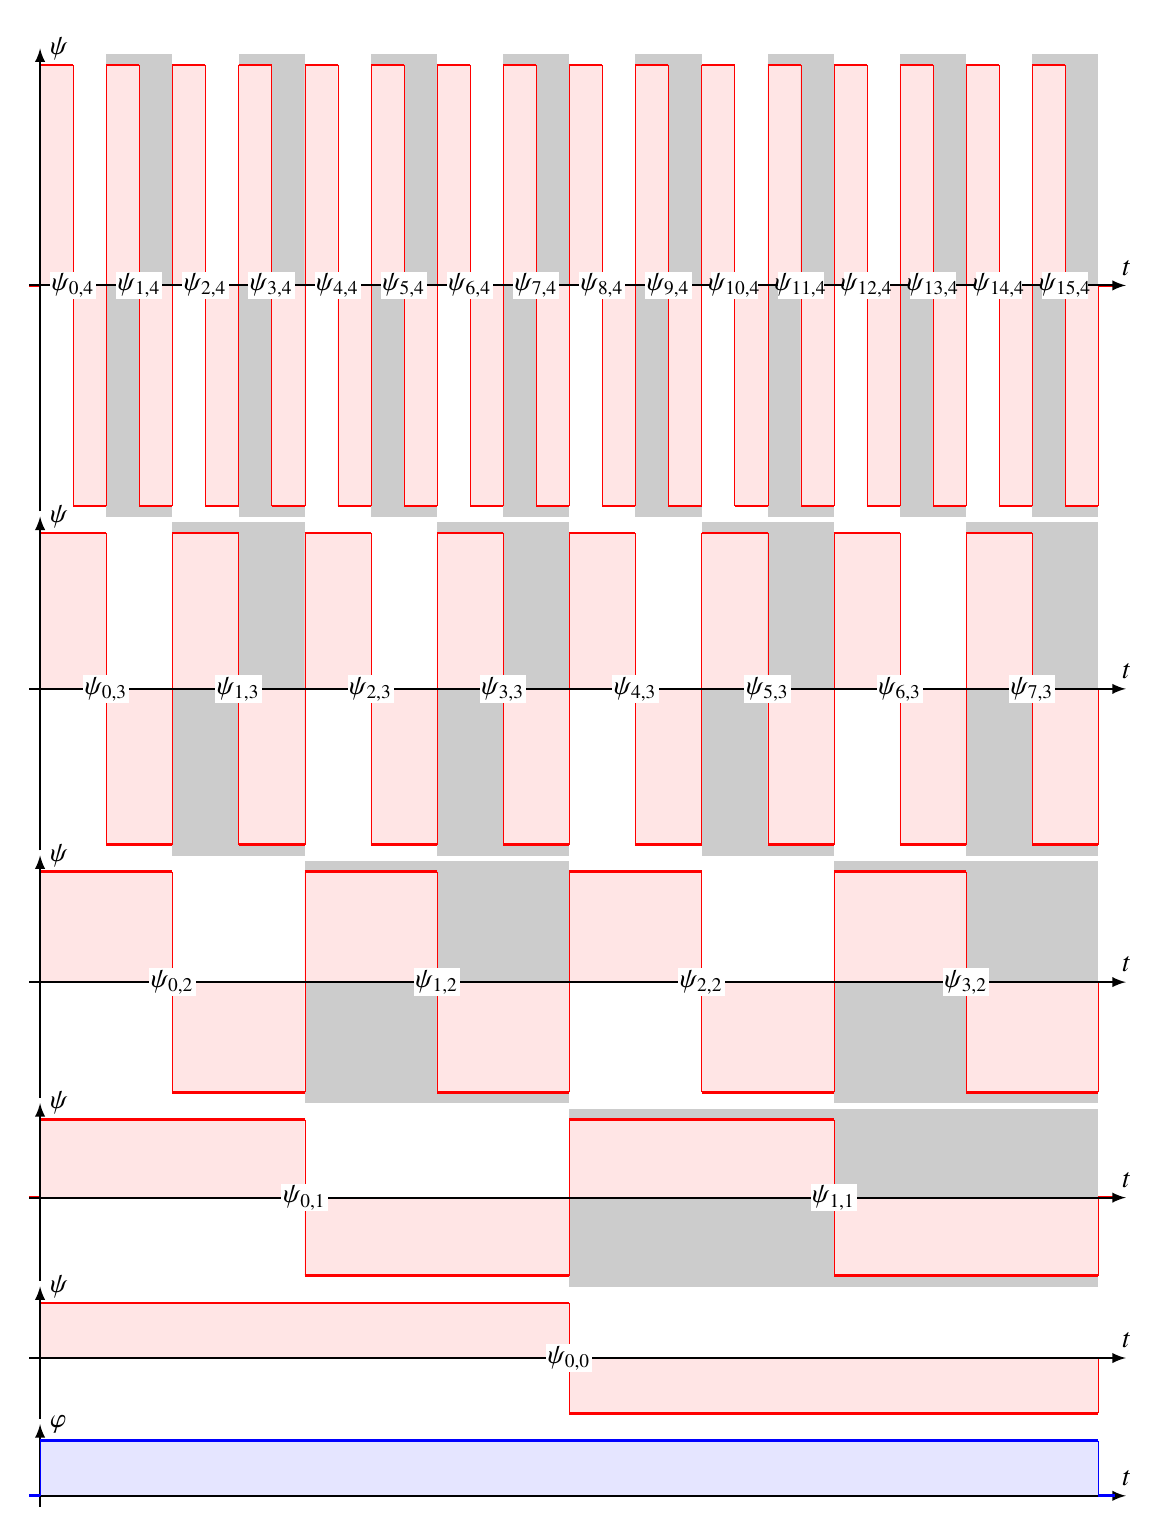
\begin{tikzpicture}[>=latex,scale=0.70]

\def\a{1.2}

\def\schatten#1#2#3{
	\fill[color=gray!40]
		({(#1)*\a*#2},{-#3-0.2}) rectangle ({(#1+2)*\a*#2},{#3+0.2});
}

%
% #1    number of steps from beginning
% #2	length in units of \a
% #3	amplitude
%
\def\welle#1#2#3{
	\fill[color=red!10] ({#1*\a*#2},0)--({#1*\a*#2},{#3})
		--({(#1+1)*\a*#2},{#3})
		--({(#1+1)*\a*#2},{-#3})
		--({(#1+2)*\a*#2},{-#3})
		--({(#1+2)*\a*#2},0)--cycle;
	\draw[line width=0.1pt,color=red]
		({#1*\a*#2},0)--({#1*\a*#2},{#3});
	\draw[line width=1pt,color=red]
		({#1*\a*#2},{#3})--({(#1+1)*\a*#2},{#3});
	\draw[line width=0.1pt,color=red]
		({(#1+1)*\a*#2},{#3})--({(#1+1)*\a*#2},{-#3});
	\draw[line width=1pt,color=red]
		({(#1+1)*\a*#2},{-#3})--({(#1+2)*\a*#2},{-#3});
	\draw[line width=0.1pt,color=red]
		({(#1+2)*\a*#2},{-#3})--({(#1+2)*\a*#2},0);
}
%
% #1 index j
% #2 Schrittweite
% #3 index k
%
\def\psikj#1#2#3{
	\fill[color=white] ({(#1+0.5)*\a*#2-0.42},-0.25)
		rectangle ({(#1+0.5)*\a*#2+0.42},0.25);
	\node at ({(#1+0.5)*\a*#2},0) {$\psi_{#1,#3}$};
}

\begin{scope}[yshift=0.5cm]
\fill[color=blue!10] (0,0)--({16*\a},0)--({16*\a},1)--(0,1)--cycle;
\draw[->,line width=0.7pt] (-0.2,0)--({16*\a+0.5},0) coordinate[label=$t$];
\draw[->,line width=0.7pt] (0,-0.2)--(0,1.3) coordinate[label={right:$\varphi$}];
\draw[line width=1pt,color=blue] (-0.2,0)--(0,0);
\draw[line width=0.1pt,color=blue] (0,0)--(0,1);
\draw[line width=1pt,color=blue] (0,1)--({16*\a},1);
\draw[line width=0.1pt,color=blue] ({16*\a},1)--({16*\a},0);
\draw[line width=1pt,color=blue] ({16*\a},0)--({16*\a+0.3},0);
\end{scope}

\begin{scope}[yshift=3cm]
\draw[line width=1pt,color=blue] (-0.2,0)--(0,0);
\welle{0}{8}{1}
\draw[line width=1pt,color=blue] ({16*\a},0)--({16*\a+0.3},0);
\draw[->,line width=0.7pt] (-0.2,0)--({16*\a+0.5},0) coordinate[label=$t$];
\draw[->,line width=0.7pt] (0,{-1-0.1})--(0,{1+0.3})
	coordinate[label={right:$\psi$}];
\psikj{0}{16}{0}
\end{scope}

\begin{scope}[yshift=5.91cm]
\draw[line width=1pt,color=red] (-0.2,0)--(0,0);
\schatten{2}{4}{sqrt(2)}
\foreach \i in {0,2}{
	\welle{\i}{4}{sqrt(2)}
}
\draw[line width=1pt,color=red] ({16*\a},0)--({16*\a+0.3},0);
\draw[->,line width=0.7pt] (-0.2,0)--({16*\a+0.5},0) coordinate[label=$t$];
\draw[->,line width=0.7pt] (0,{-sqrt(2)-0.1})--(0,{sqrt(2)+0.3})
	coordinate[label={right:$\psi$}];
\foreach \j in {0,1}{
	\psikj{\j}{8}{1}
}
\end{scope}

\begin{scope}[yshift=9.82cm]
\draw[line width=1pt,color=red] (-0.2,0)--(0,0);
\foreach \i in {2,6}{
	\schatten{\i}{2}{2}
}
\foreach \i in {0,2,4,6}{
	\welle{\i}{2}{2}
}
\draw[line width=1pt,color=red] ({16*\a},0)--({16*\a+0.3},0);
\draw[->,line width=0.7pt] (-0.2,0)--({16*\a+0.5},0) coordinate[label=$t$];
\draw[->,line width=0.7pt] (0,{-2-0.1})--(0,{2+0.3})
	coordinate[label={right:$\psi$}];
\foreach \j in {0,1,2,3}{
	\psikj{\j}{4}{2}
}
\end{scope}

\begin{scope}[yshift=15.14cm]
\draw[line width=1pt,color=red] (-0.2,0)--(0,0);
\foreach \i in {2,6,...,14}{
	\schatten{\i}{1}{2*sqrt(2)}
}
\foreach \i in {0,2,...,14}{
	\welle{\i}{1}{2*sqrt(2)}
}
\draw[line width=1pt,color=red] ({16*\a},0)--({16*\a+0.3},0);
\draw[->,line width=0.7pt] (-0.2,0)--({16*\a+0.5},0) coordinate[label=$t$];
\draw[->,line width=0.7pt] (0,{-2*sqrt(2)-0.1})--(0,{2*sqrt(2)+0.3})
	coordinate[label={right:$\psi$}];
\foreach \j in {0,1,...,7}{
	\psikj{\j}{2}{3}
}
\end{scope}

\begin{scope}[yshift=22.46cm]
\draw[line width=1pt,color=red] (-0.2,0)--(0,0);
\foreach \i in {2,6,...,30}{
	\schatten{\i}{0.5}{4)}
}
\foreach \i in {0,2,...,30}{
	\welle{\i}{0.5}{4)}
}
\draw[line width=1pt,color=red] ({16*\a},0)--({16*\a+0.3},0);
\draw[->,line width=0.7pt] (-0.2,0)--({16*\a+0.5},0) coordinate[label=$t$];
\draw[->,line width=0.7pt] (0,{-4-0.1})--(0,{4+0.3})
	coordinate[label={right:$\psi$}];
\foreach \j in {0,1,...,15}{
	\psikj{\j}{1}{4}
}
\end{scope}

\end{tikzpicture}
\end{document}

